\hyphenation{
}

Das wichtigste Kriterium für die Archivierung und Nachnutzbarkeit von Daten ist neben technischen Aspekten, wie die Wahl eines geeigneten Langzeitformates, eine vollständige Dokumentation . Viele Dokumente und Dateien sind nicht aus sich selbst heraus verständlich. Sie stehen immer in einem gewissen Forschungs- oder Projektkontext, der für die Nachnutzung dokumentiert werden muss. Damit Forschungsdaten von Dritten gefunden und sinnvoll verwertet werden können, müssen sie durch zusätzliche Informationen ergänzt und strukturiert beschrieben werden. Wenn Daten ausreichend fachlich wie technisch beschrieben werden, können sie durch andere Personen wissenschaftlich nachgenutzt werden und besitzen somit einen Wert für die Zukunft. Nur dann lohnt sich auch der Aufwand einer analogen oder digitalen Langzeitarchivierung.

Die Dokumentation eines Projektes und der erzeugten Daten sollte als ein wichtiger, kontinuierlicher Prozess verstanden werden, der von Anfang an berücksichtigt und während des gesamten Lebenszyklus von Daten umgesetzt wird -- und nicht erst nach Abschluss von Arbeiten oder bei der Übergabe von Beständen an ein Archiv. Insofern bedarf es innerhalb von größeren Projekten eines Verantwortlichen oder einer Organisationsform aller Beteiligten, welche die Struktur und Pflege der Dokumentation konzeptionell und koordinierend begleitet. Gemeinsam muss definiert werden, welcher Gegenstand dokumentiert wird, in welchem Umfang und mit welcher Gliederung, welche Form geeignet ist (z. B. Wiki versus PDF), wie die Aktualität der Inhalte erhalten wird, wie Nutzer über Änderungen informiert werden usw. Fehlende Strategien für den Aufbau und die Pflege einer Dokumentation führen häufig zu Unübersichtlichkeit und dadurch zu einer Konfusion der beteiligten Akteure. Von umfassenden, detaillierten und strukturierten Angaben zu  digitalen Daten profitieren nicht nur die Archive und zukünftige Generationen von Forschern, sondern auch die Wissenschaftler selbst während der Durchführung eines Projektes -- genauso wie es auch bei einer guten analogen Dokumentenablage der Fall ist.

Welche Informationen sind für eine Dokumentation erforderlich? Wichtig sind alle Angaben, die den Entstehungsprozess und -kontext sowie die Konventionen von Inhalten und Daten beschreiben oder zumindest skizzieren. Dabei kann die Dokumentation als "`Beipackzettel"' verstanden werden, der anderen Personen das Auffinden der Daten, das Verstehen der Inhalte, eine sinnvolle Wiederverwendung der Daten für weitere Forschungen ermöglicht und die Vergleichbarkeit von Daten erhöht. So ist es beispielsweise üblich, bei Fotografien das Aufnahmedatum, eine Kurzbeschreibung des abgelichteten Gegenstandes und den Fotografen anzugeben, Zeichnungen mit einem Maßstab, der geografischen Ausrichtung, dem Zeichner und einem Kurztext zu beschriften oder bei Texten einen Autor, einen Titel und ein Datum zu nennen.

Insbesondere bei digitalen Daten sind zusätzliche, spezialisierte Informationen erforderlich, die über die rein deskriptiven Angaben zu den Inhalten und zum Forschungsinteresse hinausgehen und nicht nur die primären Fragen zu \emph{"`Wer, Wie, Was, Wo, Wann und Warum?"'} beantworten. So sind technische und administrative Angaben über die Vorgehensweise der Datenerhebung und die eingesetzten Programme, mit denen die Daten erzeugt oder digitalisiert wurden, für ein späteres Auslesen, Auswerten und Interpretieren unverzichtbar. Auch wie die Daten strukturiert wurden und in welcher Beziehung Dateien zueinander stehen, muss in der Regel explizit erklärt werden. Angaben zu Qualitätssicherungsverfahren,  Änderungshistorie und Versionierung von Daten erlauben es, das empirische Vorgehen im Forschungsprozess nachzuprüfen. Zudem ist es wichtig zu erklären, wie Dritte zukünftig auf die Daten zugreifen  oder sie nutzen dürfen.

Damit unbeteiligte Personen den größeren Zusammenhang einer einzelnen Information oder eines Datenbestandes verstehen und nachvollziehen können, sollte jede Dokumentation eines Projektes mindestens folgende Punkte enthalten:
\begin{itemize}
	\item Angaben zur Fragestellung und zum Untersuchungsgegenstand
	\item Angaben zu den Projektverantwortlichen für Nachfragen
	\item Zusammenfassung der wissenschaftlichen Ergebnisse
	\item Beschreibung von Arbeitsabläufen und Methoden, vor allem bezüglich der Datenerhebung, -verarbeitung und Qualitätssicherung
	\item Auflistung der erzeugten unterschiedlichen Dokumentarten (z. B. Tagebücher, Berichte, Listen, Fotos etc.)
	\item Beschreibung von verwendeten Handbüchern, Standards, projektspezifischen Konventionen, Thesauri, Nummernsystemen etc.
	\item Auflistung der eingesetzten technischen Geräte und Programme
	\item Relevante Publikationen und wichtige Sekundärliteratur
	\item Wichtige Korrespondenzen, Verträge, Anträge etc. (ggf. in anonymisierter Form) 
	\item Bestimmungen zur weiteren freien oder eingeschränkten Verwendung von Daten
\end{itemize}

In dem Abschnitt Speicherung von Metadaten ab Seite \pageref{metadatenSpeicherung} sind weitere allgemeine Angaben zu finden. In dem Kapitel Dateiformate ab Seite \pageref{dateiformate} werden außerdem weitere notwendige Angaben abhängig vom Dateityp aufgelistet. Auch für die Anwendung von bestimmten Methoden werden gesonderte Dokumentationsangaben erforderlich, die in dem Kapitel Forschungsmethoden ab Seite \pageref{methoden} zu finden sind.


%##################################################################################

\subsection{Dokumentation mit Metadaten}
Ein spezifischer Bestandteil einer jeden Dokumentation sind Metadaten. Während die Dokumentation die Summe aller Angaben zu einem Projekt und der zugehörigen Daten umfasst und sie in Form, Inhalt, Länge und Struktur je nach fachlichen Gepflogenheiten völlig frei formuliert sein kann, sind Metadaten nach festen formalen Kriterien strukturiert (z. B. als Formulare oder Eingabemasken) und beschreiben die Eigenschaften von anderen Daten, ohne diese selbst zu enthalten.

Metadaten machen die fachlich oder organisatorisch notwendigen Kontextinformationen explizit und dienen zur Auffindung von relevanten Informationen, deren Identifikation, deren Auswahl und Verwaltung. Beispielsweise sind Fotos nur anhand der mit ihnen assoziierten beschreibenden Metadaten effizient durchsuch- und auffindbar oder Karten nur dank einer Maßstabsangabe und einer aussagekräftigen Legende wissenschaftlich nutzbar. Die National Information Standards Organization (NISO) definiert Metadaten als Werkzeuge, um Forschungsdaten nachhaltig zu organisieren, zu erschließen, zu verstehen und zu benutzen. Werden Metadaten standardisiert gespeichert, können sie auch maschinell verarbeitet werden.

Da Metadaten immer von unterschiedlichen Informationsbedürfnissen und Anwendungskontexten abhängig sind, lassen sie sich unter verschiedenen Blickwinkeln betrachten. Egal ob sie ein Forschungsvorhaben in seiner Gesamtheit oder den Inhalt eines einzelnen Dokuments beschreiben, können sie sich auf folgende Aspekte beziehen:
\begin{itemize}
	\item Deskriptive Angaben, die ein Projekt, ein Objekt oder eine Methode fachlich und inhaltlich näher beschreiben (z. B. Kurzbeschreibung eines Fotos, Laufzeit eines Forschungsvorhabens, Autor eines Textes)
	\item Strukturelle Angaben, welche die physischen oder logischen Beziehungen zwischen komplexen Objekten beschreiben (z. B. referenzierte Dateien in Zeichnungen, die Reihenfolge von Fotos oder zusammengehörige Dateien)
	\item Administrativ-rechtliche Angaben, die Rechteinhaber, Lizenzbedingungen und Zugangsregeln benennen und für die Verwaltung relevant sind (z. B. Fristen für die Veröffentlichung von Ergebnissen)
	\item Administrativ-erhaltungsbezogene Angaben, welche die Geschichte eines digitalen Objektes, also die  vorhergehenden und gegenwärtigen Zustände, nachvollziehen lassen und Erhaltungsmaßnahmen beschreiben (z. B. Angabe zur Herkunft einer Karte, Konvertierungsmaßnahmen)
	\item Technische Angaben, die Informationen zu Software und Hardware liefern (z. B. das Dateiformat eines Bildes, die Zeichenkodierung eines Textes oder technische Parameter eines Messgerätes). Sie werden benötigt, um Daten in veralteten Dateiformaten in neuere umwandeln oder um die ursprüngliche Programmumgebung mittels aktueller Technik nachbauen zu können.
\end{itemize}

Ein anderes Unterscheidungskriterium von Metadaten ist der Umfang der Daten, die sie beschreiben. Sie können sich beziehen auf:
\begin{itemize}
	\item Eine größere zusammenhängende Datensammlung (z. B. der gesamte Datenbestand eines Projektes)
	\item Eine einzelne Datei
	\item Eine einzelne Information innerhalb eines Systems (z. B. ein Datensatz in einer Datenbank)
\end{itemize}

Weiterhin können Metadaten auch angewandte Prozesse und Methoden beschreiben, um den Entstehungsprozess von Dateien und Dateikonvoluten verständlicher zu machen und Hinweise für den weiteren Umgang mit den Daten zu liefern. Im Abschnitt Metadaten in der Anwendung ab Seite \pageref{Metadaten-anwendung} werden daher Metadaten in drei Kategorien unterschieden:
\begin{itemize}
	\item Projektbezogene Metadaten, die den gesamten Datenbestand eines Projektes dokumentieren
	\item Dateibezogene Metadaten, die einzelne Dateien dokumentieren
	\item Methodenbezogene Metadaten, die angewandte Prozesse und Methoden dokumentieren
\end{itemize}

Außerdem kann bei Metadaten unterschieden werden zwischen solchen, die eine manuelle Eingabe erfordern, und solchen, die durch Systeme und Programme automatisch erzeugt werden können. Erstere können beispielsweise eine Kurzbeschreibung oder Schlagworte sein. Letztere sind Angaben wie Erstellungsdatum, Dateiname oder Einstellungen der Digitalkamera.

Während für ein laufendes Projekt nur ein Ausschnitt dieser Metadaten eine praktische Relevanz besitzt, sind für die digitale Langzeitarchivierung von Daten alle Aspekte wichtig. Einige der Metadaten können ausschließlich von beteiligten Personen frühzeitig während des Prozesses der Datenerzeugung erfasst werden, da nur sie den Inhalt, den Charakter, die Struktur, den Kontext und die Quellen der Daten kennen. Andere Metadaten dagegen lassen sich auch zu einem späteren Zeitpunkt bei der Archivierung und Veröffentlichung der Daten generieren.


%##################################################################################

\subsection{Strukturierung von Metadaten}
Die Struktur und der Umfang von Metadaten sind wesentliche Faktoren, um diese sinnvoll nutzen zu können. Die Art und Weise, wie die verschiedenen Informationen erfasst und organisiert werden, spielen dabei eine zentrale Rolle, ob sie von einer unbeteiligten dritten Person richtig verstanden werden und ob die Angaben automatisiert verarbeitet werden können. 

Um die Struktur und den Umfang von Metadaten verbindlich zu beschreiben und vorzugeben, werden Metadatenschemata verwendet. Ein Metadatenschema gibt den Inhalt und die Gliederung von Metadaten vor, also die zu verwendenden Metadaten-Kategorien. Beispielsweise kann eine Publikation mit den Attributen Autor -- Jahr -- Titel -- Reihe -- Verlag -- Erscheinungsort und Schlagworte beschrieben werden, die dann mit den entsprechenden Informationen gefüllt werden. Diese Minimalbeschreibung kann je nach Anforderungen erweitert werden, etwa um die Elemente Sprache -- Seitenzahl -- Abbildungszahl -- Auflage und ISBN-Nummer.

In einem Metadatenschema wird zudem für einzelne Informationen die Genauigkeit (die Granularität) der erwarteten Information festgelegt, also ob beispielsweise für das Attribut "`Autor"' eine freie Texteingabe ausreichend ist oder ob eine Aufteilung in die Teilattribute Anrede -- Titel -- Vorname(n) und Nachname sowie eine Referenz zu einer Personennormdatei erforderlich ist.

Für den Austausch von Metadaten zwischen verschiedenen technischen Systemen besitzen die zugrunde liegenden Schemata eine zentrale Bedeutung. Sollen Informationen aus unterschiedlichen Quellen miteinander in Beziehung gesetzt werden, so dass sie gemeinsam ausgewertet werden können, müssen die jeweils eingetragenen Werte auf der Ebene ihrer semantischen Bedeutung miteinander verknüpft und abgeglichen werden. Das heißt, dass neben dem eigentlichen Wert (z. B. die Zeichenkette "`Pompeji"') auch das Attribut angegeben werden muss, also die Eigenschaft, die durch den Wert beschrieben wird (z. B. "`Fundort"', "`Aufbewahrungsort"' oder "`Publikationsort"'). 

Für viele Bereiche, wie etwa Medienarchive, Bibliotheken oder Museen, gibt es langjährige Erfahrungen im Umgang mit Metadaten und es wurden spezifische Metadatenschemata entwickelt. Zu Beginn eines Projektes sollte geprüft werden, ob relevante Metadatenschemata bereits existieren oder sogar vorgegeben werden und bei der Erzeugung von eigenen Metadaten berücksichtigt werden sollten. Je internationaler und standardisierter ein verwendetes Schema ist, desto eher ist die Austauschbarkeit von Metadaten mit anderen Systemen gewährleistet. Sofern sich unterschiedliche Metadaten auf ein gemeinsames Metadatenschema abbilden (\emph{mappen}) lassen, können sie in ein drittes System importiert und dort gemeinsam geöffnet werden.

\begin{wrapfigure}{r}{0.5\textwidth}
  \begin{center}
    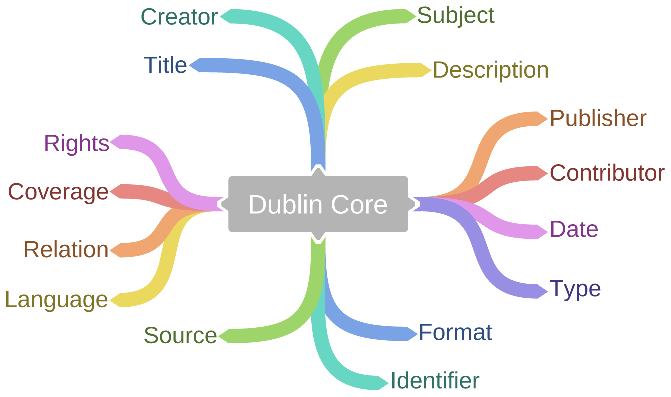
\includegraphics[width=0.5\textwidth]{bilder/doku_dublinCore}
  \end{center}
  \caption{Die 15 Kernfelder von Dublin Core Version 1.1. (Grafik erstellt mit coggle.it.)}
  \label{doku_dublinCore}
\end{wrapfigure}
Für deskriptive Metadaten ist das unter ISO 15836 zertifizierte Metadatenschema \emph{Dublin Core} (in Abbildung \ref{doku_dublinCore}) am weitesten verbreitet. Es verfügt in der Version 1.1 über folgende 15 Kernfelder: \emph{Title} (Titel) -- \emph{Creator} (Ersteller) -- \emph{Subject} (Thema) -- \emph{Description} (Beschreibung) -- \emph{Publisher} (Verleger) -- \emph{Contributor} (Mitwirkender) -- \emph{Date} (Datum) -- \emph{Type} (Typ) -- \emph{Format} (Format) -- \emph{Identifier} (Identifikator) -- \emph{Source} (Quelle) -- \emph{Language} (Sprache) -- \emph{Relation} (Beziehung) -- \emph{Coverage} (Umfang) -- \emph{Rights} (Rechte).

Im Laufe der Jahre wurde dieses grundlegende Set noch erweitert. Das aktuelle Set, "`\emph{The Dublin Core Metadata Initiative (DCMI) Metadata Terms}"', und die Beschreibung der einzelnen Attribute kann \href{http://dublincore.org/documents/dcmi-terms/}{online}\footnote{\href{http://dublincore.org/documents/dcmi-terms/}{http://dublincore.org/documents/dcmi-terms/}} abgerufen werden.

Eine besondere Relevanz im archäologischen und altertumswissenschaftlichen Kontext haben folgende Standards erlangt:
\begin{itemize}
	\item Online AccesS to the Index of archaeological investigationS (OASIS), veröffentlicht von English Heritage. Es wurde für den Nachweis von archäologischen Projekten und Maßnahmen in Großbritannien entwickelt. Das Schema liegt aktuell in Version 1.3 vor. Neben den in der Abbildung \ref{abb:doku_oasisProject} dargestellten fünf Themenbereichen können auch weitere spezielle Angaben wie etwa zu Arealen, Geophysik, Geologie und Artefakten gemacht werden.
	\begin{figure}[h!bt]
		\begin{center}
			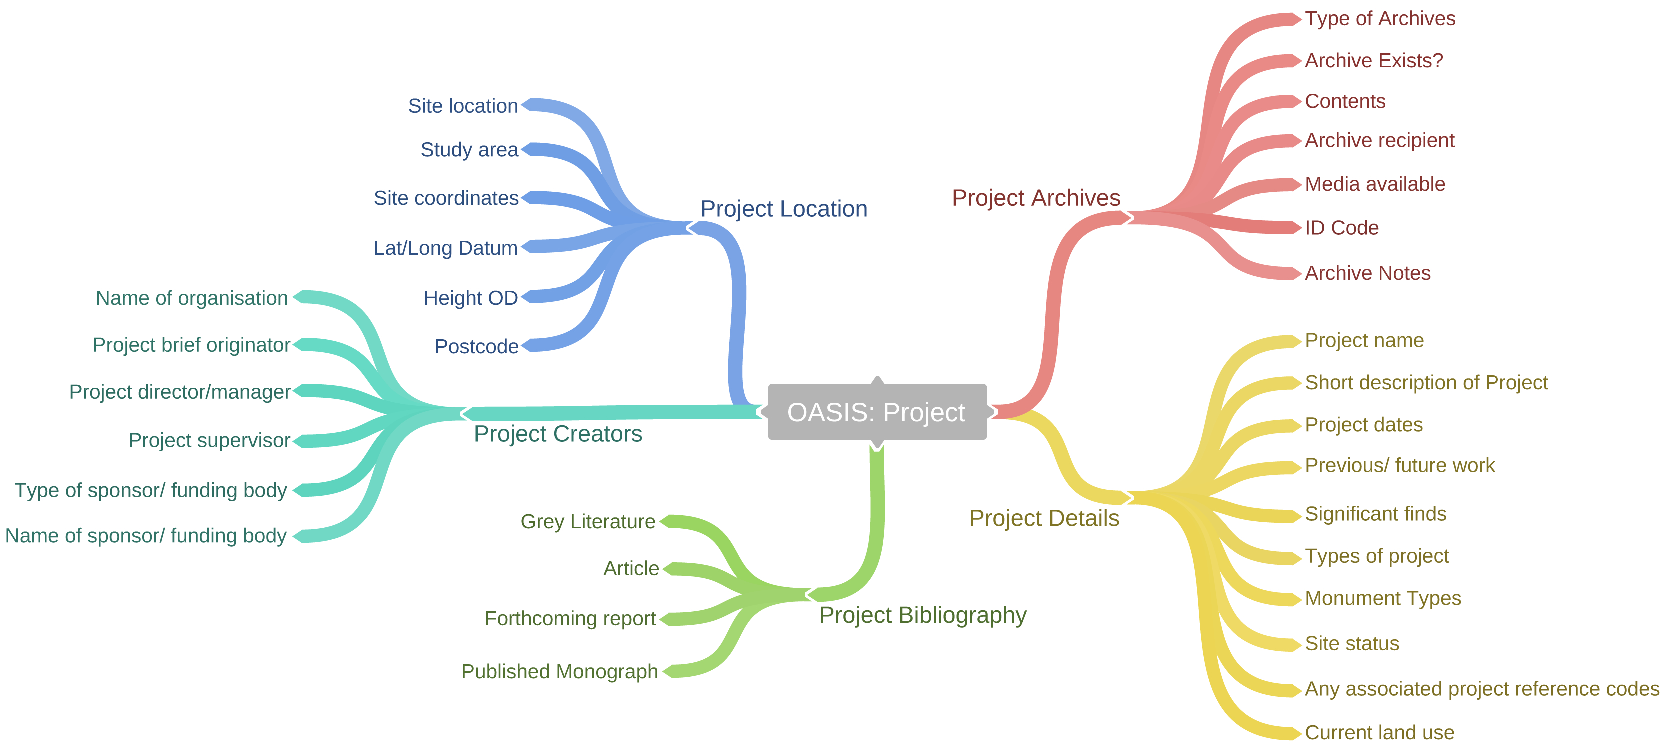
\includegraphics[width=\textwidth]{bilder/doku_oasisProject}
		\end{center}
		\caption{OASIS in Version 1.3. Neben den abgebildeten Themenbereichen sind auch Attribute für weitere spezialisiertere Informationen vorgesehen. (Grafik erstellt mit coggle.it.)}
		\label{abb:doku_oasisProject}
\end{figure}
	\item Archäologischer DateneXport-Standard (ADeX), wurde von der "`Kommission Archäologie und Informationssyteme"' beim Verband der Landesarchäologen entwickelt. Der Standard wurde für den Austausch archäologischer Fachdaten zwischen Landesämtern und anderen Institutionen erarbeitet. Die aktuelle in Abbildung \ref{abb:doku_ADeX} dargestellte Version ist 2.0, die auch den Austausch von komplexen Geometrien mittels externer Geometriedaten (SHP oder MIF) ermöglicht. ADeX ist bewusst als einfaches Austauschformat mit den Teilen "`Generelles"', "`Georeferenz"' und  "`Typ und Zeit"' unter Berücksichtigung internationaler Standards, wie etwa CIDOC-CRM, gestaltet. Dies gewährleistet eine hohe Austauschbarkeit.
	\begin{figure}[h!bt]
		\begin{center}
			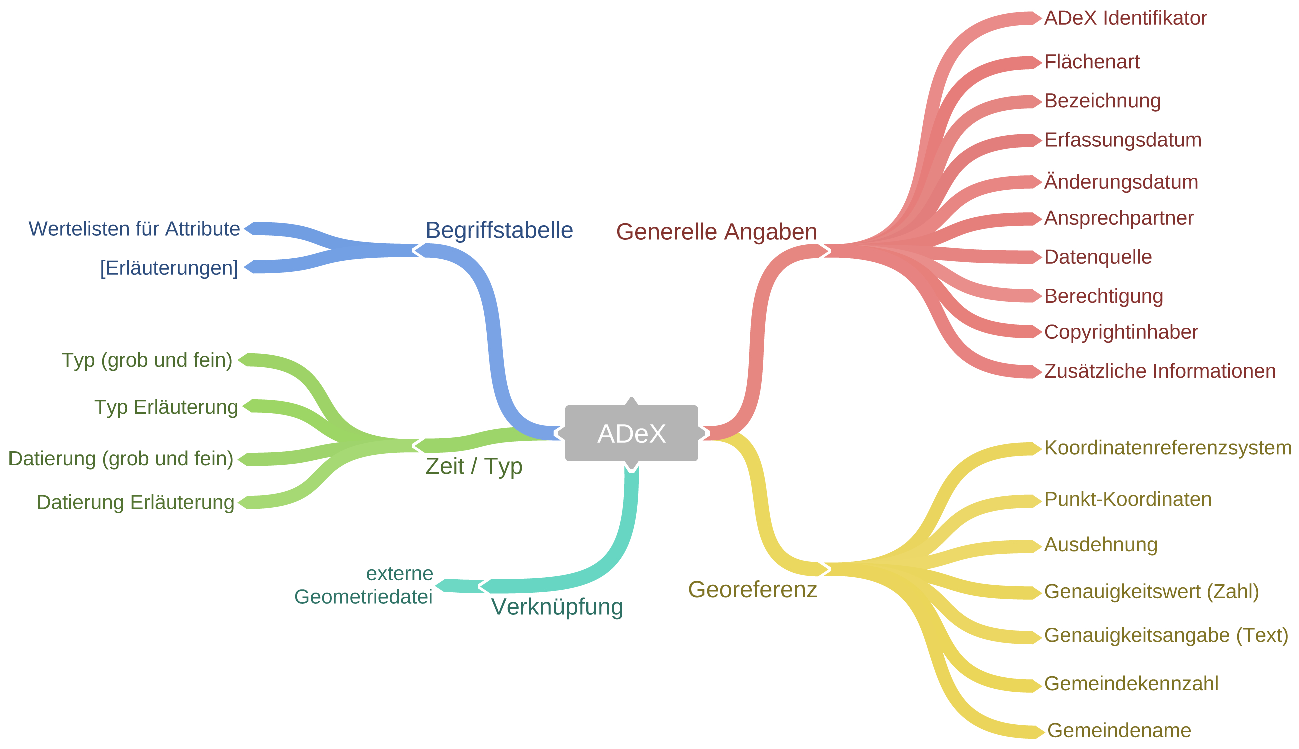
\includegraphics[width=\textwidth]{bilder/doku_ADeX}
		\end{center}
		\caption{ADeX in Version 2.0, das für eine hohe Kompatibilität auf detailliete Informationen verzichtet. (Grafik erstellt mit coggle.it.)}
		\label{abb:doku_ADeX}
\end{figure}
	\item Connecting Archaeology and Architecture in Europeana (CARARE) in Version 2.0. Es wurde als archäologiespezifisches Datenmodell unter Berücksichtigung verschiedener europäischer Standards von Europeana und dem Project 3D-ICONS entwickelt. Die Abbildung \ref{abb:doku_CARARE} verdeutlicht, dass in dem Schema Informationen zur Sammlung (\emph{Collection information}), zum physischen Objekt (\emph{Heritage asset}), zur digitalen Ressource (\emph{Digital resource}) und zur Aktivität (\emph{Activity}) definiert werden.
	\begin{figure}[h!tb]
		\begin{center}
			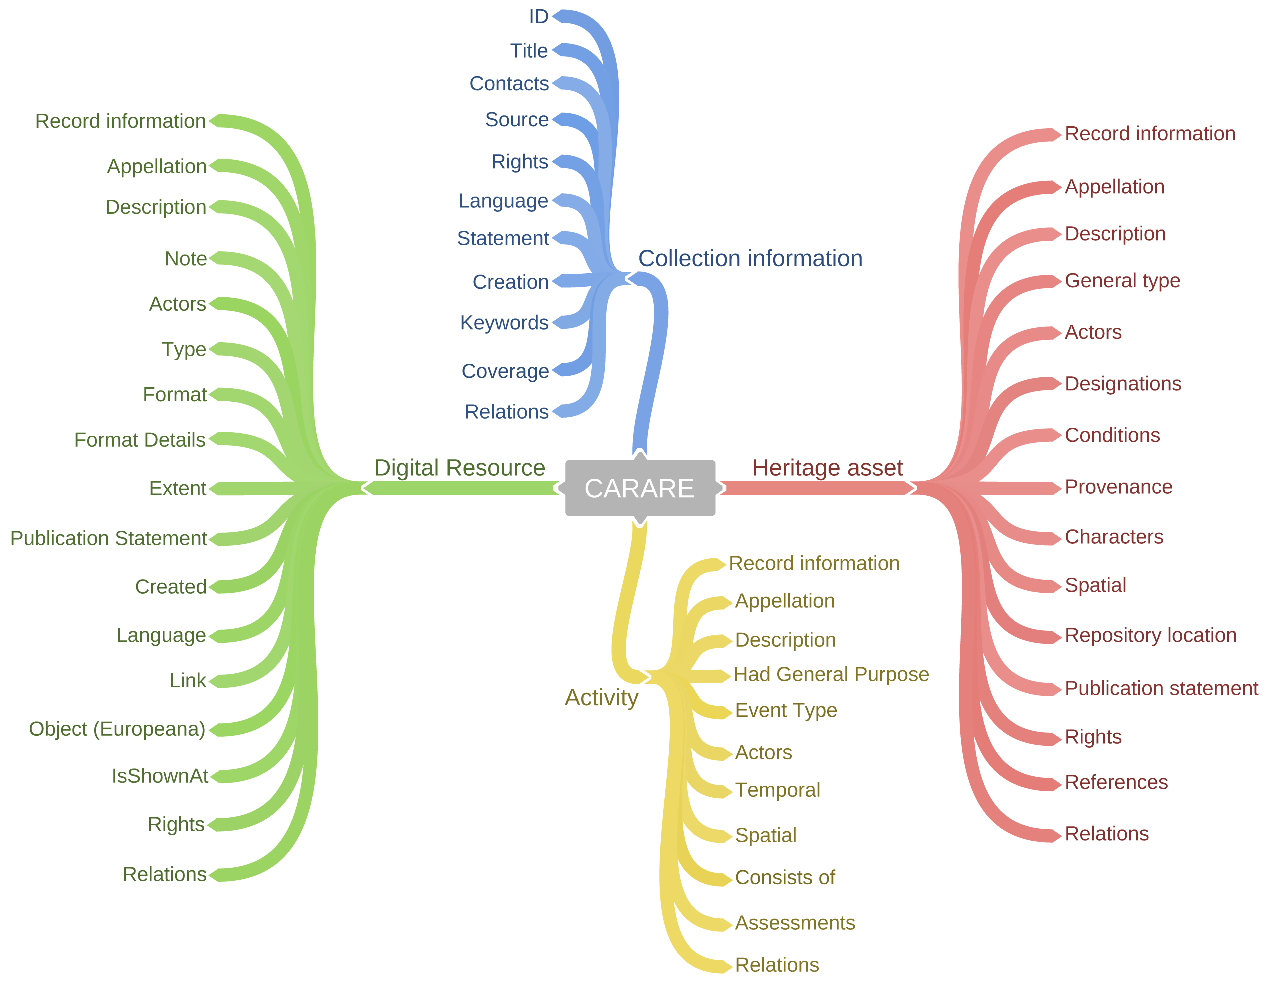
\includegraphics[width=0.9\textwidth]{bilder/doku_CARARE}
		\end{center}
		\caption{CARARE 2.0. (Grafik erstellt mit coggle.it.)}
		\label{abb:doku_CARARE}
\end{figure}
\item Das Metadatenschema von IANUS in Abbildung \ref{abb:doku_IANUS} wurde ebenfalls für Daten aus dem Bereich der Archäologien und Altertumswissenschaften entwickelt und orientiert sich an bereits vorhandenen Standards.
\begin{figure}[h!bt]
		\begin{center}
			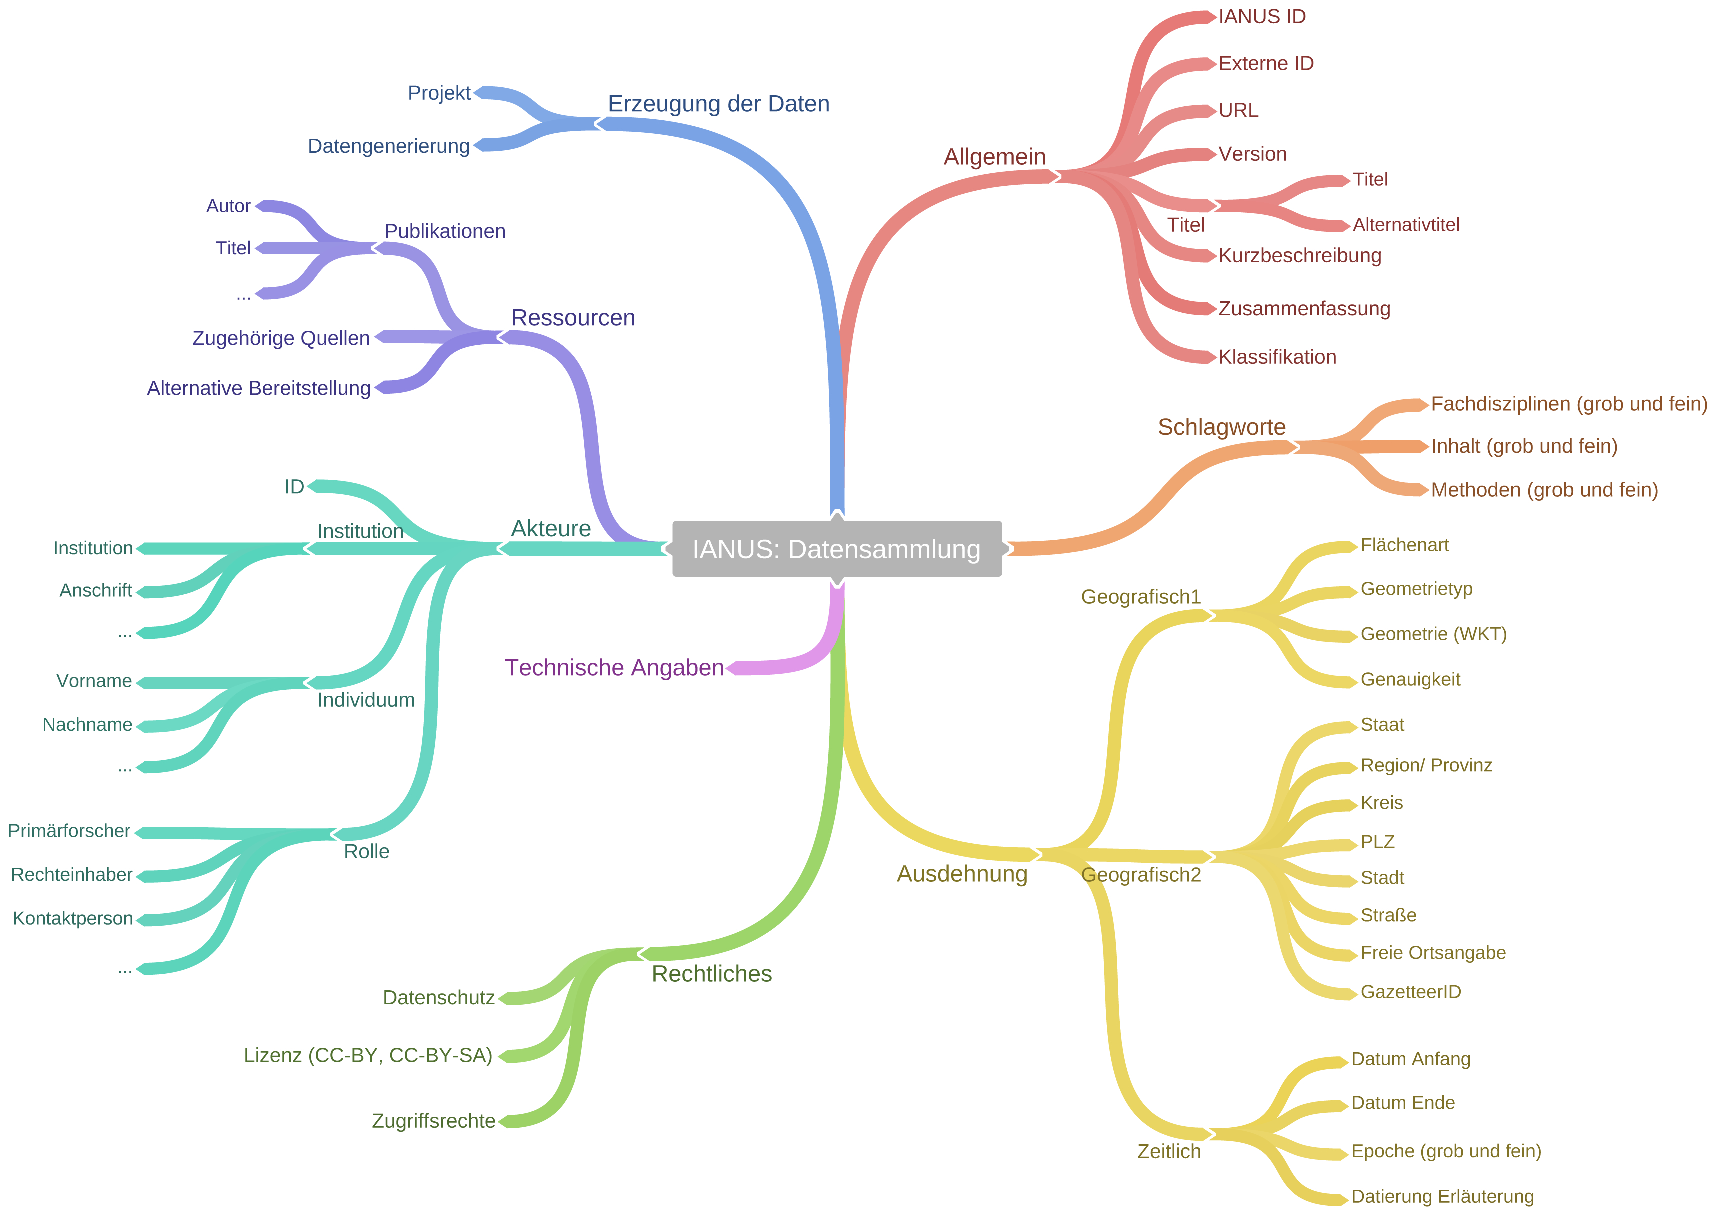
\includegraphics[width=\textwidth]{bilder/doku_IANUS}
		\end{center}
		\caption{Eine vereinfachte Darstellung des Metadatenschemas von IANUS. (Grafik erstellt mit coggle.it.)}
		\label{abb:doku_IANUS}
\end{figure}
\end{itemize}

Darüberhinaus gibt es weitere internationale Standards und institutionelle Vorgaben:
\begin{itemize}
	\item CIDOC Conceptual Reference Modell (CIDOC CRM) wurde von der Arbeitsgruppe "`Dokumentationsstandards"' im Internationalen Komitee für Dokumentation (CIDOC) des internationalen Museumsverbandes (ICOM) erarbeitet. Es dient der Strukturierung und formalen Beschreibung von Informationen, Konzepten und Relationen im Bereich des Kulturerbes. Seit 2006 ist CIDOC CRM unter ISO 21127 standardisiert. Für CIDOC-CRM gibt es zusätzlich die im Rahmen von ARIADNE entwickelten Erweiterungen CRMarchaeo, CRMba, CRNdig und CRMgeo, die eine Relevanz für die Archäologie haben. Sie werden in dem Ariadne Reference Model zusammengefasst.
	\item Das Lightweight Information Describing Objects (LIDO) wurde als Austauschformat für bewegliche Objekte in Museen von Arbeitsgruppen innerhalb von CIDOC entwickelt.
	\item Historic Environment Records oder MIDAS Heritage aus Großbritannien.
	\item Vorgaben verschiedener Denkmalämter. Weitere Informationen dazu sind in dem Abschnitt "`Grabungsdokumentation"' ab Seite \pageref{grabungsdokumentation} zu finden.
\end{itemize}


%##################################################################################

\subsection{Kontrollierte Vokabulare, Thesauri und Normdaten}
Damit Metadaten möglichst sinnvoll genutzt und maschinell verarbeitet werden können, sollten neben klar definierten Metadatenschemata auch möglichst einheitliche Begriffe und homogene Beschreibungen verwendet werden. Nur wenn gleiche Dinge auch mit den gleichen Begriffen benannt werden, ist es möglich vollständige und präzise Suchergebnisse zu erhalten oder vergleichbare Daten richtig miteinander zu verknüpfen. Die Vorgabe und Definition von festen Begriffen und Regeln hilft zudem, Mehrdeutigkeiten und Redundanzen zu vermeiden, etwa wenn eine Zeichenkette verschiedene Bedeutungen besitzen kann (z. B. Abakus als Rechenhilfsmittel oder als architektonischer Abschluss eines Kapitells), ein identischer Sachverhalt durch unterschiedliche Worte erfasst werden kann (z. B. Survey und Oberflächenbegehung) oder die Form der Angabe variieren kann (z. B. ein Datum in der Form 12.03.2012 oder 2012-03-12).
 
Das geeignete Mittel zur Vereinheitlichung der sprachlichen Vielfalt sind sogenannte kontrollierte oder normierte Vokabulare, die entweder einfache Wortlisten oder strukturierte Thesauri sein können, in denen Wörter zusammen mit ihrem semantischen Kontext verwaltet werden. Diese "`terminologische Kontrolle"' kann in unterschiedlicher Weise systematisiert und implementiert sein. 

Beispielsweise können innerhalb eines Projektes alle zu verwendenden Begriffe unter allen Beteiligten abgestimmt, klar fachlich definiert, voneinander abgegrenzt und in strukturierter Form dokumentiert werden. Diese Absprachen können dann in einem zentralen Textdokument als Projektleitfaden abgelegt oder in einer Datenbank als Felder umgesetzt werden, die nur eine begrenze Auswahl von Begriffen zur Beschreibung eines spezifischen Sachverhaltes zulassen (z. B. für das Attribut Filmart nur die Werte "`Diapositiv (Farbe)"', "`Negativfilm (Farbe)"', "`Negativfilm (SW)"' und "`Digital"').

Besser eignen sich jedoch etablierte, standardisierte, globale Vokabulare, Thesauri oder Normdateien. Sie weisen oft eine thematische, fachspezifische oder institutionelle Ausprägung auf und werden von maßgeblichen Einrichtungen kontinuierlich gepflegt. Dazu gehören beispielsweise Normdateien zur Katalogisierung aus dem Bibliotheksbereich, Personennormdateien oder Thesauri zur eindeutigen Identifizierung von geografischen Orten oder Zeitbegriffen. 

Diese globalen Systeme bieten nicht nur eine feste Bezeichnung und eine Definition eines Begriffes oder des diesem zugrunde liegenden Konzeptes, sondern auch alternative und gegebenenfalls mehrsprachige Benennungen und eine eindeutige Kennung zur Identifizierung des Begriffes. So kann beispielsweise der Ort "`Alexandria"' (\href{http://www.geonames.org/361058/alexandria.html}{361058}) in Ägypten von dem Ort "`Alexandria"' (\href{http://www.geonames.org/4744091/alexandria.html}{4744091}) in den USA mittels der in den Klammern angegebenen Kennungen aus GeoNames unterschieden werden.

Bereits existierende Thesauri und Vokabulare sollten bei der Vergabe von Metadaten berücksichtigt und angewendet werden, um den späteren elektronischen Austausch, also die Interoperabilität, der eigenen Daten mit anderen Systemen erheblich zu vereinfachen. Wenn Ressourcen in mehreren Sprachen vorliegen und entsprechend multilingual beschrieben werden sollen, müssen die genutzten Wörterbücher, Thesauri und Schlagwortsysteme äquivalente Begriffe in mehreren Sprachen abbilden.

Für die systematische Erfassung archäologischer und allgemeiner Begriffe existieren folgende Vokabulare:
\begin{itemize}
	\item Art \& Architecture Thesaurus (AAT) wurde Ende der 1970er von dem Getty Research Institute entwickelt, um die Katalogisierungsprozesse in Kunstbibliotheken und im Museumsbereich zu unterstützen und zu vereinheitlichen. Dieser Thesaurus wird von einer breiten Fachgemeinschaft kuratiert.
	\item Heritage Data -- Linked Data Vocabularies for Cultural Heritage führt die in England genutzten Vokabulare im Bereich kulturelles Erbe zusammen. 
	\item Wortnetz Kultur (WNK) wurde vom Landschaftsverband Rheinland ins Leben gerufen, um die Inhalte in deren verschiedenen Informationssystemen zu vereinheitlichen. Mittlerweile sind die Themen Kulturlandschaft, Archäologie, Kulturanthropologie, Denkmalpflege sowie Kunstgeschichte mit rund 15.000 Begriffen vertreten.
	\item Das DAI bietet mit iDAI.vocab (auch archwort) ein flaches multilinguales Vokabular mit Links auf den AAT. Außerdem gibt es mit dem iDAI.the"-sau"-rus ein System, das die Schlagworte aus den unterschiedlichen Thesauri der Bibliotheken zusammenführt und strukturiert.
	\item Die Encyclopedia of Life stellt eine weltweite Datenbank für Pflanzen und Lebewesen dar, die zusätzlich Fotos, Verbreitungskarten und Literaturhinweise enthält.
	\item In Wikidata werden alle strukturierten Daten aus den Systemen von WikiMedia erfasst und mit eindeutigen Identifikatoren zur Verfügung gestellt.
\end{itemize}

Für die eindeutige Identifizierung von geografischen Orten eignen sich, neben den amtlichen Gemeindekennzahlen und dem geodätischen Parameterdatensatz EPSG, folgende Ortsthesauri, sogenannte Gazetteers:
\begin{itemize}
	\item GeoNames ist ein Gazetteer, in dem vor allem moderne Orte, deren alternative Bezeichnungen und geografischen Koordinaten systematisch erfasst werden. Die Inhalte stammen von engagierten Nutzern weltweit.
	\item Getty Thesaurus of Geographic Names (TGN) wurde 1987 von dem Getty Research Institute ins Leben gerufen, um ebenfalls deren Katalogisierungsprozesse in Kunstbibliotheken und im Museumsbereich zu unterstützen und zu vereinheitlichen.
	\item Das DAI betreibt mit dem iDAI.gazetteer einen Gazetteer für die eindeutige Adressierung von antiken Orten, in dem außerdem auch die Eintragungen in GeoNames berücksichtigt werden.
	\item Pleiades ist ebenfalls ein Gazetteer für antike Orte mit einem Schwerpunkt auf der griechischen und römischen Antike, dessen Inhalt durch jeden Nutzer erweitert oder korrigiert werden kann.
\end{itemize}

Auch für Zeitbegriffe gibt es kontrollierte Vokabulare:
\begin{itemize}
	\item PeriodO ist ein Gazetteer für Zeitepochen. Neben der zeitlichen Information wird auch die geografische Verbreitung der jeweiligen Epoche erfasst.
	\item iDAI.chronontology ist ein vom DAI durchgeführtes Projekt, das wie PeriodO zeitliche und geografische Informationen miteinander in Beziehung setzt.
\end{itemize}

Zur Erfassung von Informationen zu Personen oder Institutionen sollten Normdateien verwendet werden, wie beispielsweise:
\begin{itemize}
	\item Das Virtual International Authority File (VIAF) kombiniert Normdateien mehrerer Nationalbibliotheken und speichert Informationen zu Personen und Institutionen, sowie deren Publikationen.
	\item Die Open Researcher and Contributor ID (ORCID) ist eine alphanumerische Zeichenkette, die der eindeutigen Identifizierung wissenschaftlicher Autoren dient. ORCID wird von einem gemeinnützigen Gremium betrieben und Autoren müssen sich selbst registrieren, um eine ID zu bekommen.
	\item Die Gemeinsame Normdatei (GND) der Deutschen Nationalbibliothek dient primär der Katalogisierung in Bibliotheken. Neben Informationen zu Personen und Körperschaften werden auch weitere Informationen zu Konferenzen, Geografika, Sachschlagwörtern und Werktiteln verwaltet.
\end{itemize}

Wenn in Metadaten auf Publikationen verwiesen werden soll, eignen sich folgende Systeme:
\begin{itemize}
	\item Die Internationale Standardbuchnummer (engl. \emph{International Standard Book Number}, ISBN) wird zur eindeutigen Identifizierung von Publikationen verwendet. Sie ist vor allem im Buchhandel verbreitet. Für Reihen und Zeitschriften wird eine ähnliche Nummer, die ISSN (Internationale Standardnummer für fortlaufende Sammelwerke, engl. \emph{International Standard Serial Number}) verwendet.
	\item Für in Deutschland veröffentlichte Medienwerke gibt es eine Ablieferungspflicht bei der Deutschen Nationalbibliothek, weshalb die dort vergebenen  eindeutigen Kennungen ebenfalls zur Identifizierung verwendet werden können.
	\item Für archäologische und altertumswissenschaftliche Publikationen eignen sich auch die Identifikatoren aus iDAI.bibliography (Zenon), in dem die umfangreichen Bestände aller DAI Bibliotheken nachgewiesen werden.
\end{itemize}

%##################################################################################
\label{metadatenSpeicherung}
\subsection{Speicherung von Metadaten}
Für eine strukturierte Speicherung von Metadaten gibt es verschiedene Möglichkeiten und Wege, die einerseits von dem Zeitpunkt (synchron mit der Datenerhebung oder im Nachhinein) und andererseits von der Art der Metadatenerfassung (manuell oder automatisiert) abhängen. 

Grundsätzlich sollten Metadaten so früh wie möglich, also bereits bei der Generierung von neuen digitalen Objekten oder am Anfang eines neuen Forschungsvorhabens vergeben werden, auch wenn diese noch nicht vollständig angegeben werden können. Somit wird vermieden, dass Informationen im Nachhinein nicht mehr nachgetragen werden können, da sie vergessen wurden oder sich nicht mehr ermitteln lassen. Eine regelmäßige Aktualisierung und kontinuierliche Metadatenpflege ist ratsam und für manche Daten, wie etwa 3D-Scans oder Geodaten auch erforderlich.

Abhängig vom verwendeten Dateiformat können Metadaten auch direkt in eine Datei integriert werden. Dies kann teilweise automatisiert erfolgen, wie beispielsweise bei digitalen Fotos. Hier werden von der Kamera automatisch technische Angaben zu Dateiformat, Verschlusszeit, Blendenöffnung, Farbinformationen usw. direkt in der Bilddatei hinterlegt. Je nach Gerät können über die Voreinstellungen auch deskriptive Informationen wie Fotograf, Aufnahmedatum, Land etc. hinzugefügt werden. Ähnliche Verfahren zur automatischen Metadatenerzeugung sind auch bei Vermessungsgeräten üblich. Die durch Geräte generierten Metadaten werden unmittelbar in einem besonderen Bereich und auf standardisierte Weise in der resultierenden Datei gespeichert, etwa bei Fotos im Format Exif im Header der Datei.

Mit Hilfe von editierbaren Dateieigenschaften können auch in anderen Dateiformaten, wie etwa DOCX, ODT oder PDF, Metadaten direkt im Header gespeichert werden. Dabei ist jedoch eine manuelle Eingabe mit Hilfe der passenden Software erforderlich. Diese Informationen können über die Eigenschaften einer Datei angezeigt und teilweise verändert und ergänzt werden, was in Abbildung \ref{eigenschaftenAcrobat} für ein PDF-Dokument zu sehen ist. Bei der Auswahl von Anwendungen sollte darauf geachtet werden, ob diese spezifischen Metadaten entweder als separate Datei exportiert oder ob sie mit den Dateien, in denen sie enthalten sind, auch unabhängig von der ursprünglichen Software geöffnet werden können.

\begin{figure}[t!]
  \begin{center}
    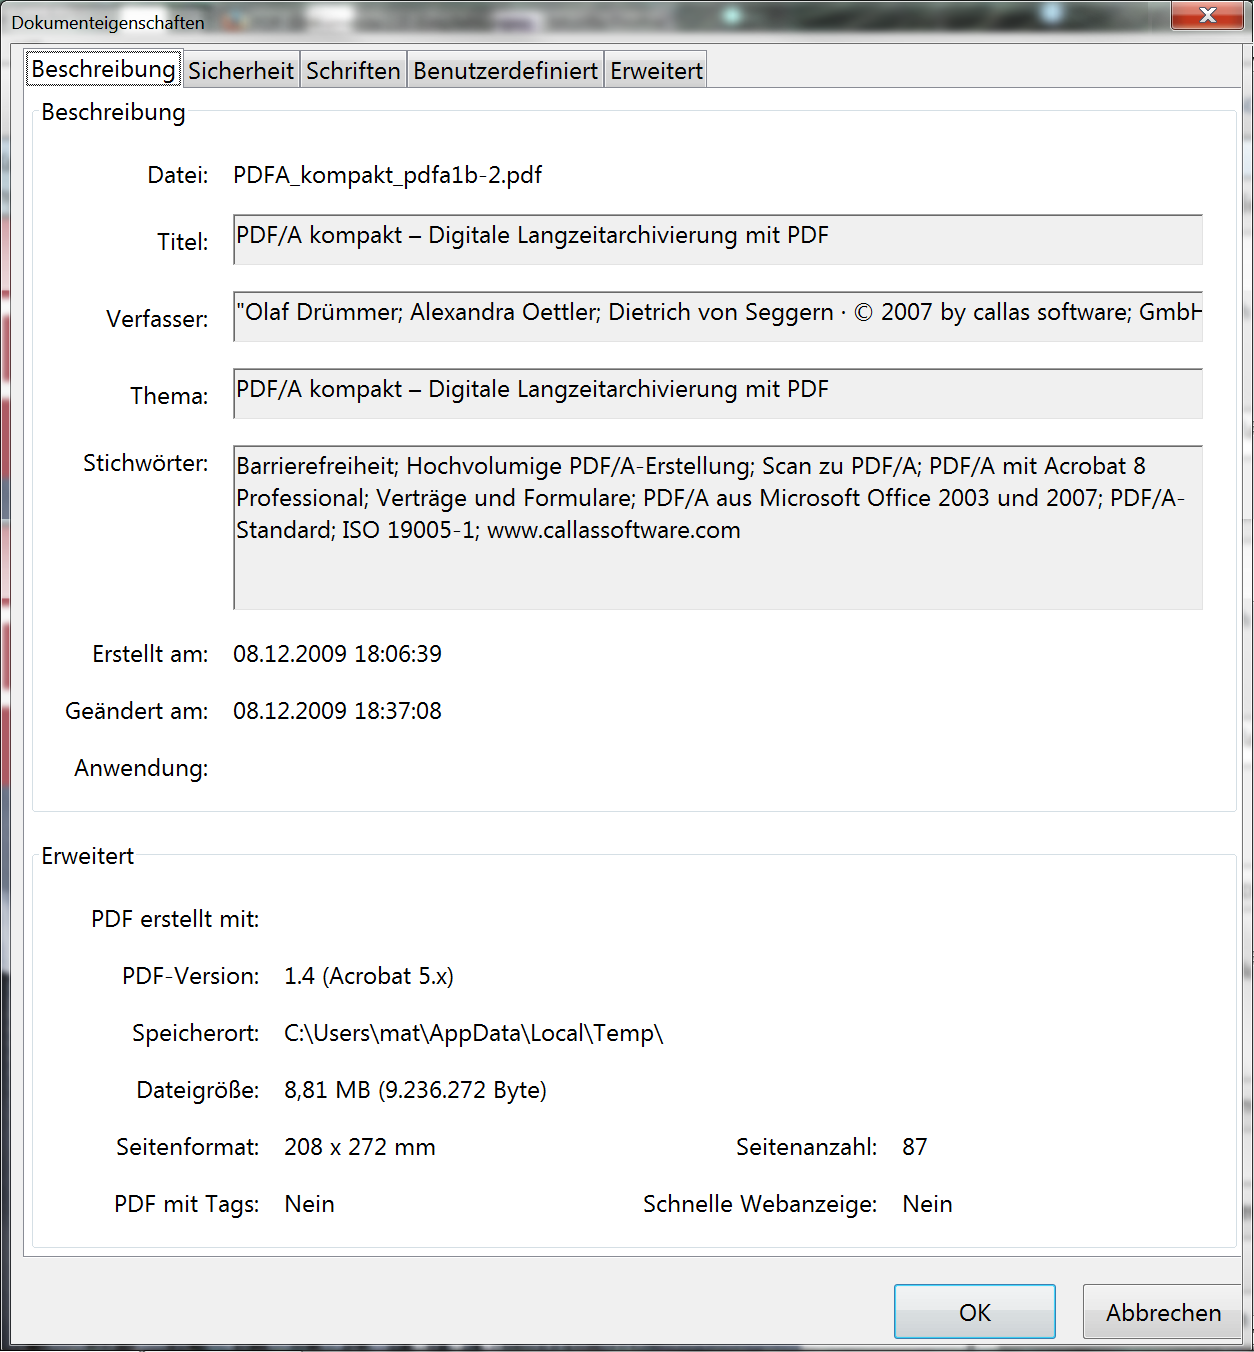
\includegraphics[width=0.9\textwidth]{bilder/doku_AdobeEigenschaften}
  \end{center}
  \caption{Beispiel der Metadaten eines PDF-Dokumentes im Programm Adobe Reader. Die Metadaten können unter "`Datei > Eigenschaften"' angezeigt und verändert werden.}
  \label{eigenschaftenAcrobat}
\end{figure}

Bei textbasierten (insbesondere XML-basierten) Dateiformaten oder Textdateien, die Auszeichnungssprachen verwenden (wie etwa SVG-, HTML- oder XML-Dateien), können Metadaten leicht mittels Auszeichnungselementen im Header der Datei integriert werden. Konkrete Hinweise für die Bearbeitung und Ergänzung von Metadaten für bestimmte Dateiformate sind in den entsprechenden Abschnitten im Kapitel Dateiformate ab Seite \pageref{dateiformate} zu finden. Auch Hinweise für die Extraktion von Metadaten in separate Dateien sind ebenfalls in den entsprechenden Abschnitten zu finden.

Für Dateiformate, in denen kein eigener Metadatenbereich vorgesehen ist, oder für übergeordnete projekt- und methodenbezogene Metadaten, ist eine Speicherung in separaten Dateien oder Systemen erforderlich. Hierfür eignen sich Tabellen und Datenbanken, da diese die Erfassung mithilfe spezifischer Eingabemasken, einer gezielten Suche und einer strukturierten Sicherung von Metadaten erleichtern. Zusätzlich erlauben sie eine (Teil-)Automatisierung der Metadaten, wie etwa die automatische Speicherung des Datums der letzten Bearbeitung eines Datensatzes und den Namen des Bearbeiters. Ein weiterer Vorteil der Erfassung von Metadaten in Tabellen oder Datenbanken besteht in der effizienten Bearbeitung von Merkmalen, die für mehrere Dokumente identisch sind, wie beispielsweise der gleiche Maßstab für alle Zeichnungen eines Projektes.

Bei der Speicherung von Metadaten in separaten Dateien muss in besonderer Weise darauf geachtet werden, dass die Beziehungen zwischen beiden Einheiten eindeutig und aktuell sind. Wird etwa bei den Metadaten der Name einer Datei zur Identifizierung verwendet, muss sichergestellt werden, dass dieser einmalig ist (ggf. in Kombination mit seinem Speicherort) und dass im Falle der Umbenennung der Datei der Eintrag auch bei den Metadaten aktualisiert wird.

Die Erfassung von Metadaten in einer Freitextdatei sollte vermieden werden, da diese meist nicht automatisiert durch Computer überprüft und verarbeitet werden können.

Bei Dokumenten mit Textinhalt können beschreibende Metadaten auch automatisch erzeugt werden, indem nach charakteristischen Zeichenketten gesucht wird und Schlag- und Stichworte extrahiert werden. Allerdings reicht die Qualität einer automatischen Erschließung bislang nicht an eine manuelle und intellektuelle Metadatenvergabe heran, da maschinell nicht nur sinnvolle Deskriptoren herausgefiltert werden.

Für die Übergabe von Dateien und Metadaten an ein Langzeitarchiv gilt die Empfehlung, die Metadaten sowohl in den Originaldateien selbst als auch in einem separaten, strukturierten und textbasierten Dokument vorzuhalten: in den Originaldateien selbst, um keine verwaisten, also undokumentierten Werke zu erzeugen, und als separate Textdatei, um eine automatisierte Verarbeitung und den Austausch von Referenzangaben zu vereinfachen.